\chapter{Anwendungsbeispiele}   
Dieses Kapitel gliedert sich in verschiedene Unterkapitel, in denen jeweils einzelne Anwendungsbeispiele der Singulärwertzerlegung näher beschrieben werden.
In ausgewählten Beispielen wird zusätzlich mithilfe der Programmiersprache \texttt{Python} eine eigene, simplifizierte Art der Anwendung konstruiert.
Grundkenntnisse in \texttt{Python} werden bei den Erklärungen des Programmcodes vorausgesetzt, es wird folglich nicht auf jede Zeile im Code genau eingegangen.

\section{Hauptkomponentenanalyse}

Die Hauptkomponentenanalyse (engl.\ \textit{Principal Component Analysis}, PCA) ist ein Verfahren zur Dimensionsreduktion von Daten.
Genauer: Es handelt sich um eine Methode, um komplexe Daten auf ihr Wesentliches zu reduzieren, was eine Weiterverarbeitung und Visualisierung erleichtert.

In diesem Unterkapitel wird zunächst die Intuition hinter der PCA erläutert, bevor der mathematische Hintergrund und insbesondere die Verbindung zur Singulärwertzerlegung beschrieben wird.
Abschließend betrachten wir ein konkretes Anwendungsbeispiel und berechnen dies mithilfe von \texttt{Python}.
Die Intuition und Mathematik orientiert sich dabei zum Großteil an~\cite[S.~165-169]{ngMachineLearningCS2292023}.

\subsection{Intuition der PCA}
Angenommen, es sei eine Datenmatrix
\begin{equation*}
    \big[
        \begin{matrix}
            x_1 \dots x_d
        \end{matrix}    
    \big] \in \R^{n \times d},
\end{equation*}
gegeben, wobei die Spaltenvektoren \(x_i \in \R^{n}\) für \(i \in \{1,\ldots,d\}\) die Ausprägung von \(d\) Merkmalen über \(n\) Objekte hinweg repräsentieren.
In \zcref{fig:pcadim}, zu finden in \zcref{appen}, wird dies für verschiedene Werte von \(d\) veranschaulicht.
Sollen die Objekte auf Ähnlichkeit bezüglich der verschiedenen Merkmale untersucht werden, kann dies im zwei- und dreidimensionalen Raum durch die grafischen Darstellungen erfolgen, indem betrachtet wird, wie sich die Punkte im Raum gruppieren.
In höheren Dimensionen ist diese visuelle Interpretation jedoch nicht mehr möglich, es besteht also die Notwendigkeit, die Anzahl der Merkmale zu verringern.

Die Hauptkomponentenanalyse bietet dafür die Möglichkeit, indem neue, unkorrelierte Komponenten konstruiert werden, die sich als Linearkombination aus den bestehenden Merkmalen zusammensetzen.
Das Ziel der Analyse ist, die Daten auf eine niedrigere Dimension zu projizieren und gleichzeitig ein Minimum an Informationen zu verlieren, also eine maximale Streuung oder auch Varianz der Daten zu erhalten.

Um dieses Konzept näher zu verdeutlichen, betrachte \zcref{fig:pca2d}.
\begin{figure}[bt]
    \centering
    \begin{subfigure}{\textwidth}
        \centering
        \caption{}\label{fig:pca2d1}
        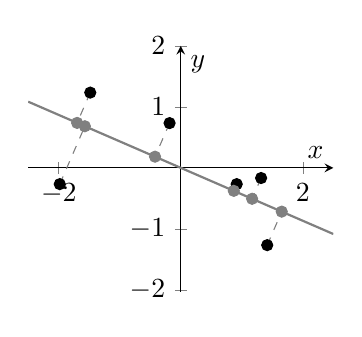
\begin{tikzpicture}[baseline]
        \begin{axis}[
            xlabel={\(x\)},
            ylabel={\(y\)},
            axis y line=center,
            axis x line=middle,
            axis equal,
            width=0.45\textwidth,
            xmin=-2.5,
            xmax=2.5
        ]
        \addplot[only marks,mark options={fill=black, color=black},domain=-2:2] coordinates {
            (1.4167,-1.2667)
            (-1.4833,1.2333)
            (1.3167,-0.1667)
            (-1.9833,-0.2667)
            (0.9167,-0.2667)
            (-0.1833,0.7333)                
        };
        \addplot[Gray, thick, domain=-2.5:2.5] {-0.4337*x};

        \addplot[only marks, mark options={fill=Gray, color=Gray}] coordinates {
            ( 1.65481157, -0.71762599)
            (-1.69867778,  0.73664903)
            ( 1.16912424, -0.50700271)
            (-1.57200891,  0.68171777)
            ( 0.86894276, -0.37682593)
            (-0.42195053,  0.18298317)
        };
        \addplot[dashed, gray] coordinates {
            (1.4167, -1.2667) ( 1.65481157, -0.71762599)
        };
        \addplot[dashed, gray] coordinates {
            (-1.4833, 1.2333) (-1.69867778,  0.73664903)
        };
        \addplot[dashed, gray] coordinates {
            (1.3167, -0.1667) ( 1.16912424, -0.50700271)
        };
        \addplot[dashed, gray] coordinates {
            (-1.9833, -0.2667) (-1.57200891,  0.68171777)
        };
        \addplot[dashed, gray] coordinates {
            (0.9167, -0.2667) (0.86894276, -0.37682593)
        };
        \addplot[dashed, gray] coordinates {
            (-0.1833, 0.7333) (-0.42195053,  0.18298317)  
        };
        \end{axis}
    \end{tikzpicture}
        \hspace{20pt}
        \begin{tikzpicture}[baseline]
    \begin{axis}[
        xlabel={\(PC1\)},
        ylabel={},
        axis y line=center,
        axis x line=middle,
        axis equal,
        ytick=\empty,
        width=0.45\textwidth,
        xmin=-2.5,
        xmax=2.5
    ]
    \addplot[only marks, mark options={fill=black, color=black}] coordinates {
        ( 1.803, 0)
        (-1.849, 0)
        ( 1.279, 0)
        (-1.697, 0)
        ( 0.928, 0)
        (-0.469, 0)
    };


    \end{axis}
\end{tikzpicture}
    \end{subfigure}
    \begin{subfigure}{\textwidth}
        \centering
        \caption{}\label{fig:pca2d2}
        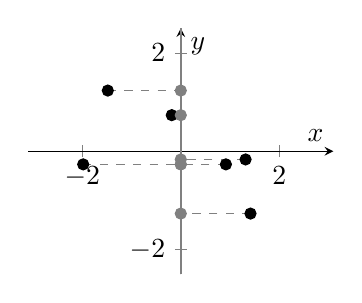
\begin{tikzpicture}[baseline]
    \begin{axis}[
        xlabel={\(x\)},
        ylabel={\(y\)},
        axis y line=center,
        axis x line=middle,
        axis equal,
        width=0.45\textwidth,
        xmin=-2.5,
        xmax=2.5
    ]
    \addplot[only marks,mark options={fill=black, color=black},domain=-2:2] coordinates {
        (1.4167,-1.2667)
        (-1.4833,1.2333)
        (1.3167,-0.1667)
        (-1.9833,-0.2667)
        (0.9167,-0.2667)
        (-0.1833,0.7333)                
    };
    \addplot[Gray, thick, domain=-2.5:2.5] ({0}, x);

    \addplot[only marks, mark options={fill=Gray, color=Gray}] coordinates {
        (0,-1.2667)
        (0,1.2333)
        (0,-0.1667)
        (0,-0.2667)
        (0,-0.2667)
        (0,0.7333)
    };
    \addplot[dashed, gray] coordinates {
        (1.4167, -1.2667) (0,-1.2667)
    };
    \addplot[dashed, gray] coordinates {
        (-1.4833, 1.2333) (0,1.2333)
    };
    \addplot[dashed, gray] coordinates {
        (1.3167, -0.1667) (0,-0.1667)
    };
    \addplot[dashed, gray] coordinates {
        (-1.9833, -0.2667) (0,-0.2667)
    };
    \addplot[dashed, gray] coordinates {
        (0.9167, -0.2667) (0,-0.2667)
    };
    \addplot[dashed, gray] coordinates {
        (-0.1833, 0.7333) (0,0.7333)  
    };
    \end{axis}
\end{tikzpicture}
        \hspace{20pt}
        \begin{tikzpicture}[baseline]
    \begin{axis}[
        xlabel={\(PC1\)},
        ylabel={},
        axis y line=center,
        axis x line=middle,
        axis equal,
        ytick=\empty,
        width=0.45\textwidth,
        xmin=-2.5,
        xmax=2.5
    ]
    \addplot[only marks, mark options={fill=black, color=black}] coordinates {
        (-1.2667,0)
        (1.2333,0)
        (-0.1667,0)
        (-0.2667,0)
        (-0.2667,0)
        (0.7333,0)
    };


    \end{axis}
\end{tikzpicture}
    \end{subfigure}
    \caption{Projektionen im zweidimensionalen Raum}\label{fig:pca2d}
\end{figure}
Bei der Frage, ob durch die Projektion in \zcref{fig:pca2d1} oder durch die in \zcref{fig:pca2d2} mehr Informationen bezüglich der Ähnlichkeit der verschiedenen Punkte bewahrt werden, ergibt sich die intuitive Antwort, dass \zcref{fig:pca2d1} vorzuziehen ist.
Trotz der Reduktion der Dimensionen von zwei auf eine, bleibt die räumliche Verteilung im Wesentlichen erhalten.

Der Grund dafür ist, dass in \zcref{fig:pca2d1} eine Richtung gewählt wurde, die den durchschnittlichen Abstand der ursprünglichen Punkte zu den projizierten Punkten auf der durch die Richtung definierten Gerade minimiert.
Es wird also versucht, den Fehler (Informationsverlust) durch die Projektion so gering wie möglich zu halten.
Dies ist äquivalent dazu, den durchschnittlichen Abstand der projizierten Punkte zum Ursprung zu maximieren (dies lässt sich durch den Satz des Pythagoras herleiten), folglich bleibt die maximal mögliche Varianz der Daten erhalten.
Es sei darauf hingewiesen, dass hier davon ausgegangen wird, dass die Daten zentriert sind, der Mittelwert also null beträgt.

Die erste Hauptkomponente (PC1) stellt dann die gewählte Richtung mit maximaler Varianz dar.
In höheren Dimensionen wird die zweite Hauptkomponente orthogonal zur ersten gewählt, um die verbleibende Varianz, die durch den Fehler in der PC1 nicht erklärt wird, erneut zu maximieren.
Dies kann beliebig fortgesetzt werden, die PCA besitzt allerdings eine nützliche Eigenschaft, die dies meist nicht erforderlich macht und auf die in der mathematischen Herleitung ausführlicher eingegangen wird.

\subsection{Mathematische Herleitung}

Um die vorangegangenen Überlegungen zu formalisieren, wird zunächst die Datenmatrix
\begin{equation*}
    X = 
    \big[
        \begin{matrix}
            x_1 \dots x_d
        \end{matrix}    
    \big] \in \R^{n \times d}
\end{equation*} 
standardisiert, indem wir eine neue Matrix 
\begin{equation*}
    \overline{X} = 
        \begin{bmatrix}
            \overline{x}_1 \dots \overline{x}_d
        \end{bmatrix} \in \R^{n \times d}
\end{equation*} 
definieren mit 
\begin{equation*}
    \overline{x}_{i,j} = \frac{x_{i,j}-\mu_i}{\sigma_i} \quad \text{für } i \in \{1,\ldots,d\} \text{ und } j \in \{1,\ldots,n\},
\end{equation*}  
wobei 
\begin{equation*}
    \mu_i = \frac{1}{n}\sum_{j=1}^{n}x_{i,j}, \quad \sigma_{i}^{2} = \frac{1}{n}\sum_{j=1}^{n}{(x_{i,j} - \mu_{i})}^{2}
\end{equation*}
jeweils die Mittelwerte, bzw.\ die Varianzen der einzelnen Merkmale, also der Spalten sind.
Die Zentrierung um den Ursprung durch die Subtraktion des Mittelwerts vereinfacht dabei spätere Rechnungen erheblich, ist rein formal allerdings nicht zwingend erforderlich.
Durch die Division der Standardabweichung wird Ungenauigkeiten aufgrund verschiedener Skalen der Merkmale vorgebeugt.
Falls Merkmal A beispielsweise das Bruttoinlandsprodukt und Merkmal B die Geburtenrate verschiedener Länder darstellt, wird dadurch eine Vergleichbarkeit gewährleistet.
In den folgenden Berechnungen wird eine Standardisierung angenommen und weiterhin mit \(X\) gearbeitet.
Wir definieren 
\begin{equation*}
    \R^{d} \ni x^{(i)} \coloneqq X_{i,:} \quad \text{für } i \in \{1,\ldots,n\},
\end{equation*}
also die \(i\)-te (transponierte) Zeile von \(X\), wobei jede Zeile je einen Punkt im Raum darstellt.

Das Ziel ist, einen Einheitsvektor \(u \in \R^{d}\) zu finden, sodass nach Projektion der Vektoren \(x^{(i)}\) auf \(u\) eine maximale Varianz, also eine maximale quadratische Abweichung vom Mittelwert, erhalten bleibt.
Die Projektion eines Vektors ist gegeben durch \zcref{rep:proj}.
\begin{repitition}\label{rep:proj}
    Sei \(n \in \N\) und \(u,x \in \R^{n}\) mit \(\norm{u} = 1\).  \\
    Dann ist der orthogonal projizierte Vektor \(\operatorname{proj}_{u}(x)\) von \(x\) auf \(u\) gegeben durch
    \begin{equation*}
        \operatorname{proj}_{u}(x) = \langle x,u \rangle u = (x^{T}u)u.
    \end{equation*}     
\end{repitition}
Um die Varianz zu ermitteln wird zunächst der Mittelwert \(\mu_{\operatorname{proj}}\) der projizierten Vektoren berechnet:
\begin{equation*}
    \mu_{\operatorname{proj}} = \frac{1}{n}\sum_{i=1}^{n}\big(x^{{(i)}^{T}}u\big)u = \left({\left(\frac{1}{n}\sum_{i=1}^{n}x^{(i)}\right)}^{T}u\right)u = \symbf{0},
\end{equation*}
da durch die Standardisierung der Spaltenmittelwert für jede Spalte von \(X\) null beträgt, wodurch
\begin{equation*}
    \sum_{i=1}^{n}x^{(i)} = \symbf{0}.
\end{equation*}
Die Entfernung (Abweichung) vom Ursprung für einen beliebigen Vektor \(x^{(i)}\) beträgt
\begin{equation*}
    \norm{\operatorname{proj}_{u}\big(x^{(i)}\big)} = \norm{\big(x^{{(i)}^{T}}u\big)u} =  \abs{\big(x^{{(i)}^{T}}u\big)}\norm{u} = \abs{x^{{(i)}^{T}}u}.
\end{equation*}
Damit ist die Varianz der projizierten Punkte gegeben durch 
\begin{align*}
    \frac{1}{n}\sum_{i=1}^{n}{\big(x^{{(i)}^{T}}u\big)}^{2} &= \frac{1}{n}\sum_{i=1}^{n}x^{{(i)}^{T}}ux^{{(i)}^{T}}u \\
    &= \frac{1}{n}\sum_{i=1}^{n}u^{T}x^{(i)}x^{{(i)}^{T}}u \qquad (\text{Skalarprodukt kommutativ})\\
    &= u^{T}\left(\frac{1}{n}\sum_{i=1}^{n}x^{(i)}x^{{(i)}^{T}}\right)u
\end{align*}
Definiere 
\begin{equation*}
    \Sigma \coloneqq \frac{1}{n}\sum_{i=1}^{n}x^{(i)}x^{{(i)}^{T}} \in \R^{d \times d}.
\end{equation*}
Diese Matrix ist als \emph{Kovarianzmatrix} bekannt, in unserem Fall ist sie die Kovarianzmatrix der verschiedenen Merkmale.
Es sei angemerkt, dass \(\Sigma\) symmetrisch ist, beachte dafür:
\begin{equation*}
    \Sigma^{T} = {\left(\frac{1}{n}\sum_{i=1}^{n}x^{(i)}x^{{(i)}^{T}}\right)}^{T} = \frac{1}{n}\sum_{i=1}^{n}{\left(x^{(i)}x^{{(i)}^{T}}\right)}^{T} = \Sigma.
\end{equation*}
Damit haben wir unser Ziel auf folgendes Optimierungsproblem reduziert:
\begin{alignat*}{2}
    &\!\max \qquad &&u^{T} \Sigma u, \\
    &\text{u.d.B.}  &&\norm{u}=1.
\end{alignat*}
Dieses Optimierungsproblem wird in der Literatur meist mithilfe von Lagrange-Multiplikatoren gelöst.
In dieser Arbeit werden wir einen anderen Ansatz verfolgen und mit dem, im vorherigen Kapitel bewiesenen, Spektralsatz (\zcref{spec}) vorgehen, wobei sich an~\cite{hsuMachineLearningTheory2016} orientiert wird.

Da \(\Sigma\) symmetrisch ist, kann der Spektralsatz angewendet werden, womit 
\begin{equation*}
    \Sigma = R \Lambda R^{T}
\end{equation*}
für orthogonales \(R =
\big[
    \begin{matrix}
        r_{1}\ldots r_{d}
    \end{matrix}
\big] \in \R^{d \times d}\) und diagonales \(\Lambda = \operatorname{diag}(\lambda_1,\ldots,\lambda_d)\) mit \(\lambda_1 \geq \cdots \geq \lambda_d\).
Für \(w \coloneqq R^{T}u\) gilt dann
\begin{equation*}
    u^{T}\Sigma u = u^{T}R \Lambda R^{T} u = w^{T}\Lambda w = w^{T}
    \begin{bmatrix}
        \lambda_1 w_{1} \\
        \vdots \\
        \lambda_d w_{d}
    \end{bmatrix}
    =\sum_{i=1}^{d}\lambda_{i}w_{i}^{2}.
\end{equation*}
Nach Bedingung gilt \(\norm{u}=1\), womit:
\begin{equation*}
    \norm{w} = \norm{R^{T}u} = \sqrt{\langle R^{T}u,R^{T}u \rangle} = \sqrt{u^{T}RR^{T}u} = \norm{u} = 1.
\end{equation*} 
Da 
\begin{equation*}
    \sum_{i=1}^{d}\lambda_{i}w_{i}^{2} = \lambda_{1}w_{1} + \lambda_{2}w_{2} + \cdots + \lambda_{d}w_{d}
\end{equation*}
und \(\lambda_1 \geq \cdots \geq \lambda_d\) wird der Ausdruck maximiert für \(w = \symbf{e}_{1}\).
Es folgt
\begin{equation*}
    u = Rw = R\symbf{e}_{1} = r_{1},
\end{equation*}
womit \(u\) nach \zcref{cor:spec} gleich dem zugehörigen Eigenvektor zum größten Eigenwert von \(\Sigma\) ist.  